\documentclass[10pt]{article} 
\usepackage{graphicx}
\usepackage[T1]{fontenc}
\begin{document}
\title{Initial report on analysis of the Anganwadi dataset 2010} 
\author{Avishek Sen Gupta\\ThoughtWorks}
\maketitle
\newpage

\section{Abstract}
This report summarises the results of exploration of the Anganwadi dataset provided by the Akshara Foundation. The analysis aims to characterise the structure of the data, and reveal trends (which would otherwise be obscured by the format of the source data) which may inform strategy through subsequent prediction and/or classification procedures.

\newpage
\section{Methodology}
\subsection{CRISP-DM}
\textbf{CRISP-DM} is a process model distilled from the most common approaches used in data mining procedures. It stands for Cross Industry Standard Process for Data Mining. Not so much a prescription as a collection of 'good practices' follwed by data mining professionals, \textbf{CRISP-DM} has the following characteristics.

\begin{itemize}
\item Domain-neutral
\item Tool-neutral
\item Provides a structural approach to the data mining process
\end{itemize}

\textbf{CRISP-DM} segregates data mining endeavours into the following phases.

\begin{itemize}
\item Business Understanding
\item Data Understanding
\item Data Preparation
\item Modeling
\item Evaluation
\item Deployment
\end{itemize}

\subsection{Relevance of CRISP-DM to this report}
As far as this report is concerned, the relevant or most significant phases we focus on are:
\begin{itemize}
\item Data Understanding
\item Data Preparation
\item Modeling
\end{itemize}

Work on the Evaluation step is still preliminary, and will probably be the subject of another report. In a full-fledged project, the rest of the activities upstream and downstream to the above list will assume more importance, and require corresponding investment.

\newpage
\section{Data Preparation}
\subsection{Nature of the source data}
The dataset comes from the education domain. The source data is a file, with each line corresponding to a single student evaluation record. Roughly, there are 29000 records, prior to any data sanitisation. Each line is pipe(|)-delimited into multiple fields. The fields salient to this analysis are listed below:

\begin{itemize}
\item Location of the student's school
\item Language of the student
\item Student's score before intervention
\item Student's score after intervention
\end{itemize}

The score is not a single number, it is a set of 56 responses marked as 0/1. Generally, a 1 may be treated as a favourable answer, therefore, adding them up to get a single aggregate score has natural ordering: a sense of who did better. We reproduce two such records below, with the original formatting.\\

{\footnotesize 30915|YALLAMMANADODDI|KANNADA|1231468|Girl||1NoSection|Aug 2010 Assessment|1|1|1|1|1|1|1|1|1|1|1|1|1|1|1|1|1|1|1|1|1|1|1|1|1|1|1|1|1|1|1|1|1|1|1|1|1|1|1|1|1|1|1|1|1|1|1|1|1|1|1|1|1|1|1|1|Anganwadi Post Test|1|1|1|1|1|1|1|1|1|1|1|1|1|1|1|1|1|1|1|1|1|1|1|1|1|1|1|1|1|1|1|1|1|1|1|1|1|1|1|1|1|1|1|1|1|1|1|1|1|1|1|1|1|1|1|1|}\\

{\footnotesize 29607|BADAMAKAAN I|KANNADA|1445172|Girl|URDU|1NoSection|Aug 2010 Assessment|1|0|1|1|0|1|0|1|1|1|1|1|1|1|1|0|1|1|1|1|1|0|1|1|1|1|1|0|1|1|1|0|1|1|1|1|1|1|0|1|1|0|1|1|1|1|1|1|1|1|1|1|1|1|1|0|Anganwadi Post Test|1|0|1|1|1|0|1|1|0|1|1|0|1|1|1|1|0|1|1|1|0|0|1|1|0|1|0|0|1|1|1|0|1|1|0|0|1|1|1|0|0|1|1|1|1|1|1|1|1|1|1|1|1|1|1|1|
...
}\\

Looking at the second row, we see that the location of the Anganwadi is BADAMAKAAN I, the student is female and speaks Urdu. The first contiguous set of 0s and 1s is the pre-intervention score, and the next set is the post-intervention one.

\subsection{Data representation}
\subsubsection{Data store}
Before any sort of sanitisation or analysis may be performed, it is important to ensure that the source data is stored in a format/datastore which makes querying and modifying the data relatively painless. This decision is largely driven by technological considerations, like:

\begin{itemize}
\item Scale of data (centralised/distributed store?)
\item Sophistication of queries (OLAP/OLTP?)
\item Structure of data, or lack thereof (SQL/NoSQL?)
\end{itemize}

We were dealing with only about 29000 records, and most of the analysis would probably be performed outside the database. Thus, we opted to use MySQL as our datastore.
\subsubsection{Schema}
The decisions when creating the database schema affect the ease of querying for relevant information. Apart from the attributes of interest, we wanted to store the individual binary responses as well. One way is to create one column for each response, giving us a total of 112 columns for storing these responses (56 for pre-intervention, 56 for post-intervention). The other way, and that is the one that we chose was to store this information as a 64-bit integer (bigint for MySQL). When required, we could unpack the individual response bits from this number.\\
We elected to not create any more schema elements like reference data for area or language at this point, because we were not sure (yet) whether there was any data corruption which could lead to duplicate reference data.\\\\
A {\tt desc responses;} command on the table reveals the schema we ended up with.

{\tt
\begin{verbatim}
+------------------+------------+------+-----+---------+----------------+
| Field            | Type       | Null | Key | Default | Extra          |
+------------------+------------+------+-----+---------+----------------+
| student_id       | int(11)    | YES  |     | NULL    |                |
| area             | char(50)   | YES  |     | NULL    |                |
| pre_performance  | bigint(20) | YES  |     | NULL    |                |
| post_performance | bigint(20) | YES  |     | NULL    |                |
| language         | char(50)   | YES  |     | NULL    |                |
| gender           | char(20)   | YES  |     | NULL    |                |
| pre_total        | int(11)    | YES  |     | NULL    |                |
| post_total       | int(11)    | YES  |     | NULL    |                |
| id               | int(11)    | NO   | PRI | NULL    | auto_increment |
+------------------+------------+------+-----+---------+----------------+
\end{verbatim}
}

\subsection{Data migration: Identifying invalid data}
It is natural to expect missing or corrupted data. The most crucial attribute are the score data, as any misinterpretation of that data may adversely bias the quality of our analysis. Thus, specific checks were put in place to ensure that none of the binary responses was null or some string other than 0 or 1.\\\\
Using this check, we found 1067 responses which violated it. All of them had either empty pre- or post-intervention scores. We did not migrate these response records, though it may be possible to do Monte Carlo simulations to predict the missing data.\\
As a result, out of a total of 28535 records in the original source, 27468 were migrated to the database.\\
We also found a large fraction of records which did not have a LANGUAGE attribute, i.e., that field was empty. Nevertheless, they were included in the migration.

\newpage
\section{Bias}
Analysis is most suscpetible to bias in the data collection stage. Sampling is one such activity. If, for a statistical study, participating individuals are not equally likely to have been selected, it may be difficult to distinguish between the actual phenomenon and this biased sampling.
This sort of bias is called sampling bias.

\subsection{Sampling bias}
To find evidence for bias, we looked at a few parameters.
Here is the breakdown of the population by language, with the biggest language bucket highlighted.\\\\
Unspecified=869\\
URDU=3564\\
\textbf{KANNADA=18685}\\
TELUGU=1688\\
TAMIL=2051\\
MARATHI=91\\
OTHER=239\\
HINDI=243\\
KONKANI=18\\
GUJARATHI=12\\
NOT KNOWN=3\\
ORIYA=2\\
MULTI LNG=1\\
BENGALI=1\\
NEPALI=1\\
\\
There is an overwhelming proportion of students who speak Kannada as their mother tongue (leading by an order of magnitude), a fact that is very likely to bias any sort of analysis where language is involved. We must remain cognizant of such biases, and interpret the results accordingly.\\\\
Here is the breakdown of the population by gender.\\\\
\textbf{Girl=14822}\\
Boy=12646\\\\
There is not a huge disparity between the two sexes, which indicates that any analysis/prediction based on gender may be less biased.

\newpage
\section{Shape of the Data}
Before embarking on any deep analysis of data, it behooves us to look at the shape of the raw data. There are a few reasons why we want to do this.\\
\begin{itemize}
\item Evident trends/outliers: Visualisation of the raw data set is always a quick way to spot trends without doing too much analysis. Of course, visualisation is best suited for 1,2 and 3-dimensional data: data of higher dimensionality must usually be either sliced prior to visualisation, or have its dimensionality reduced, before projecting it onto the 2D plane.\\
Having said that, there are other ways of visualising the data without sacrificing any dimensions at all, such as Parallel Coordinates, though it is more suited to data exploration.
\item Evidence of conformance to well-known distributions: There exist many probability distributions, some of whose properties are well-studied and well-known, like the Normal distribution. If the data approximates one of these distributions, there are several mature statistical methods which may be applied to test different hypotheses and properties of the data.\\
Indeed, many of the classical statistical analyses make the assumption that the underlying data is normally distributed.
\end{itemize}

In the following sections, we shall explore the shape of the Anganwadi 2010 dataset, and record our observations on it.

\subsection{Univariate distributions}
The graph below shows 3 distributions: the pre-intervention scores, the post-intervention scores, and the improvements.\\
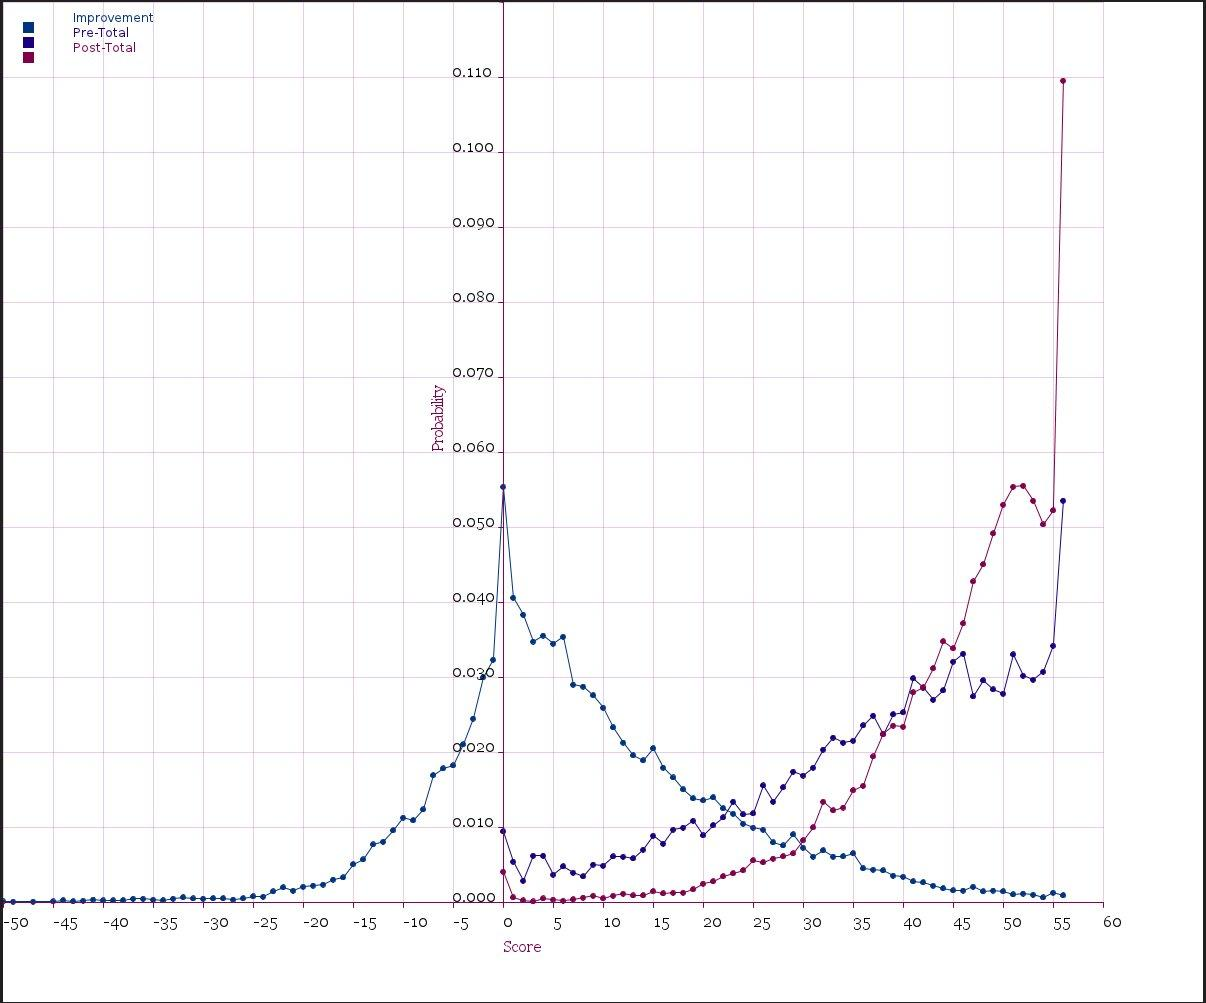
\includegraphics[width=160mm]{ReportMedia/ShapeOfData.jpg}
\subsubsection{Observations}
\begin{itemize}
\item The pre-intervention score with the highest number of students is 56, which is the highest score possible. This implies that, even prior to intervention, a sizeable fraction of the students have score very high.
\item The post-intervention score also follows the same trend, albeit with a steeper curve, which implies that many students have scored better in the post-test than in the pre-test.
\item The improvement distribution is peaked, the peak being near zero. This makes sense, because if a large fraction of students answered all 56 questions as 1 in the pre-intervention score, there really is no way for them to improve. This is assuming that their performance did not worsen in the post-test.
\item There is a significant fraction of students whose performance has worsened in the post-test. This number is 7081. Out of those, we noticed that the worsening was dramatic for a small set. We have listed down the records which had a regression of 40 or more, below.

{\tt
\begin{verbatim}
+------------+-----------------------+-----------+------------+----------+
| student_id | area                  | pre_total | post_total | language |
+------------+-----------------------+-----------+------------+----------+
|    1506619 | VABASANDRA            |        52 |          0 | KANNADA  |
|    1444355 | KITTAGANA COLONY      |        56 |          0 | KANNADA  |
|    1426910 | PRIYA DARSHINI        |        53 |          0 | KANNADA  |
|    1445387 | KYALASANAHALLI        |        51 |          1 | TELUGU   |
|    1445382 | KOTHANUR              |        44 |          0 | TAMIL    |
|    1445383 | KOTHANUR              |        41 |          0 | KANNADA  |
|    1442911 | BETTANA PALYA         |        55 |         12 | KANNADA  |
|    1445160 | KODIGEHALLI           |        52 |          0 | KANNADA  |
|    1457095 | KAVERI NAGARA         |        41 |          0 | KANNADA  |
|    1457090 | KAVERI NAGARA         |        44 |          0 | TELUGU   |
|    1457092 | KAVERI NAGARA         |        41 |          0 | TELUGU   |
|    1507686 | REHMATH NAGAR         |        44 |          0 | URDU     |
|    1448385 | MALSANDRA             |        50 |          0 | KANNADA  |
|    1455798 | KANTEERAVA COLONY     |        55 |         15 | KANNADA  |
|    1444466 | PRIYA DARSHINI        |        52 |          0 | KANNADA  |
|    1444467 | PRIYA DARSHINI        |        44 |          0 | KANNADA  |
|    1445337 | RACHENAHALLI          |        52 |          0 | KANNADA  |
|    1425269 | VINYAKNAGAR           |        41 |          0 | KANNADA  |
|     552534 | KYALASANAHALLI        |        52 |          1 | TELUGU   |
|    1448976 | KRISHNA SAGARA COLONY |        54 |         14 | KANNADA  |
|    1507157 | BELTHURU              |        52 |          7 | KANNADA  |
|    1444897 | MUNESHWARA NAGAR      |        45 |          0 | TAMIL    |
|    1444890 | MUNESHWARA NAGAR      |        40 |          0 | KANNADA  |
|    1542861 | VERABADRA NAGAR 1     |        56 |          1 | KANNADA  |
|    1358415 | KOTHANUR              |        48 |          8 |          |
|    1445437 | THRIVENINAGARA        |        40 |          0 | TELUGU   |
|    1442907 | BETTANA PALYA         |        55 |          8 | KANNADA  |
|    1457106 | KAVERI NAGARA         |        40 |          0 | TELUGU   |
|    1445444 | THRIVENINAGARA        |        41 |          0 | TELUGU   |
|    1444474 | PRIYA DARSHINI        |        54 |          0 | KANNADA  |
|    1445159 | KODIGEHALLI           |        41 |          0 | KANNADA  |
|     511998 | KODIGEHALLI           |        55 |          0 | KANNADA  |
|    1356274 | KAVERI NAGARA         |        56 |          0 |          |
|    1358429 | KOTHANUR              |        42 |          0 |          |
|    1497510 | JALAHALLI 1           |        42 |          0 | KANNADA  |
|    1443914 | BIDARAHALLI           |        56 |         12 | KANNADA  |
|    1366955 | PRIYA DARSHINI        |        53 |          0 | KANNADA  |
|    1366956 | PRIYA DARSHINI        |        53 |          0 | KANNADA  |
|    1447019 | MADAPPANA HALLI       |        42 |          0 | TELUGU   |
|    1355112 | BYRATHI BANDE         |        55 |         14 |          |
|    1504259 | MAYASANDRA  A         |        56 |          0 | KANNADA  |
|    1457120 | KAVERI NAGARA         |        43 |          0 | TAMIL    |
|    1457089 | KAVERI NAGARA         |        43 |          0 | TAMIL    |
|    1445171 | KODIGEHALLI           |        44 |          0 | KANNADA  |
|    1457203 | SARAIPALYA            |        51 |          0 | URDU     |
|    1457179 | BYRATHI BANDE         |        55 |         14 | KANNADA  |
|    1504538 | KEMPEGOWDA NAGAR      |        51 |          7 | KANNADA  |
|    1444486 | PRIYA DARSHINI        |        49 |          0 | KANNADA  |
|    1444488 | PRIYA DARSHINI        |        42 |          0 | KANNADA  |
|    1451831 | AMBED NAGAR           |        50 |          9 | TAMIL    |
+------------+-----------------------+-----------+------------+----------+
\end{verbatim}
}
\item Lololol
\end{itemize}
\subsection{Outlier Analysis}
\subsection{Bivariate distribution}
\subsection{Summary plots}
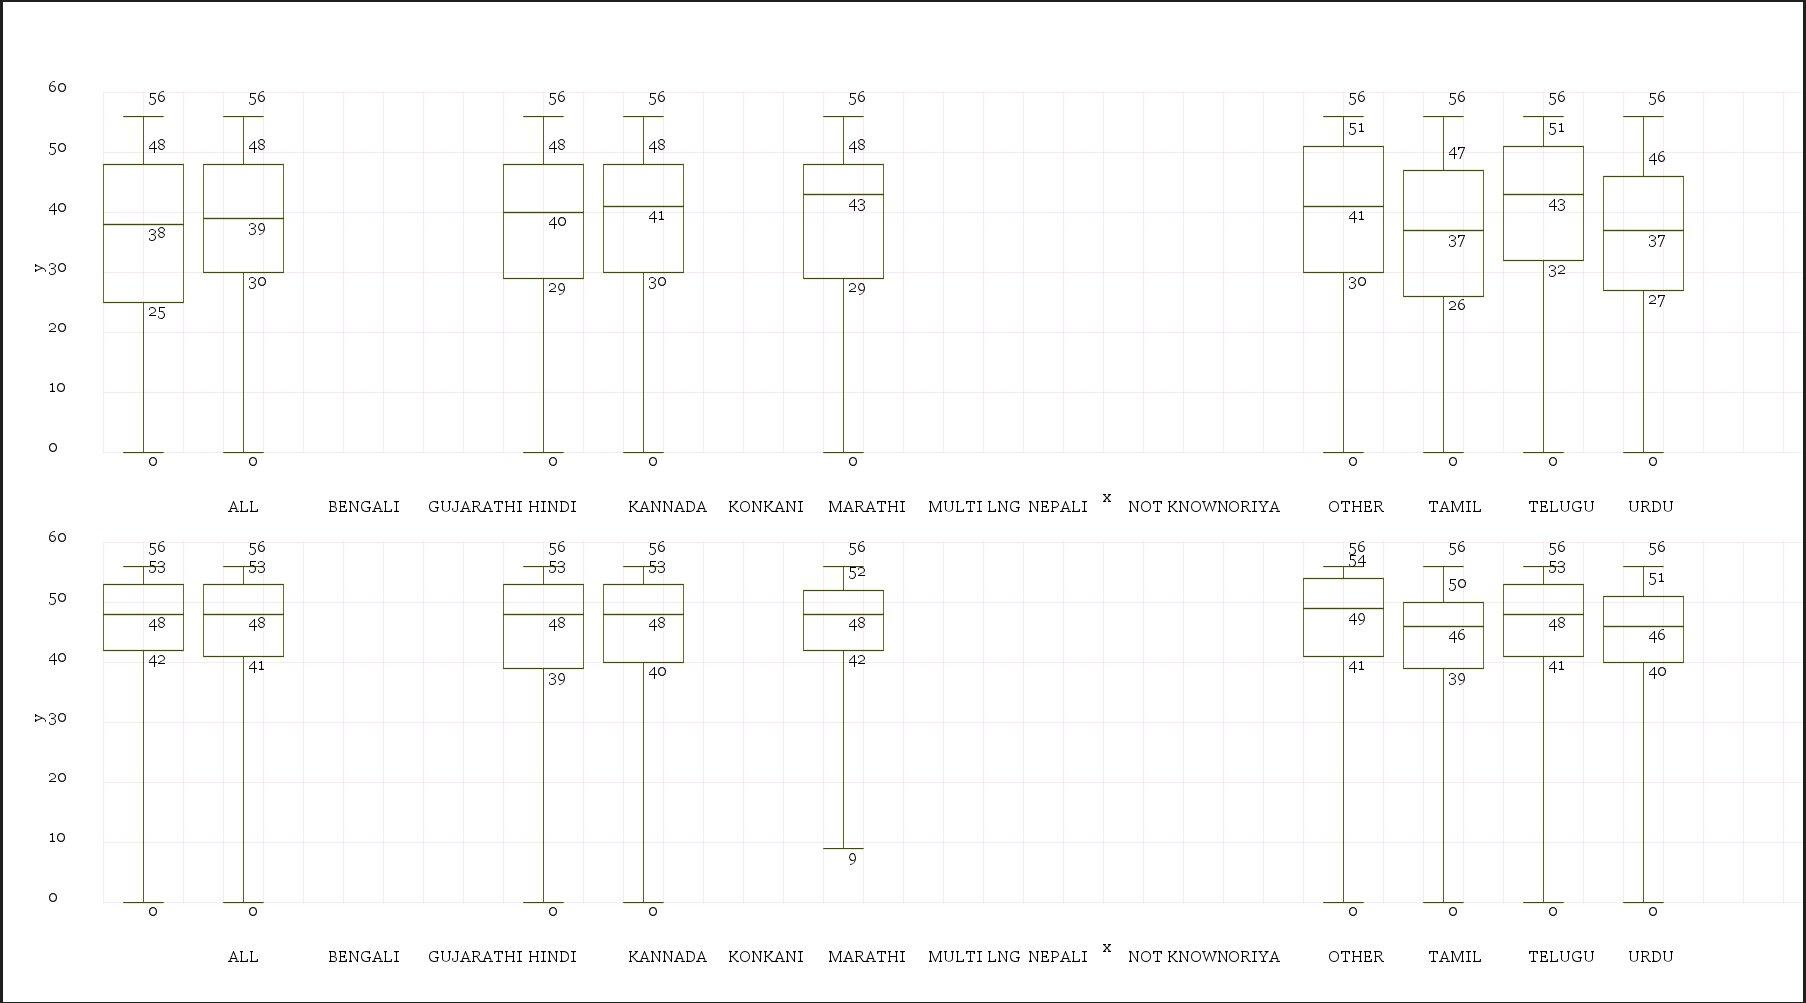
\includegraphics[width=160mm]{ReportMedia/BoxPlotPrePost.jpg}
	
\newpage
\section{Data exploration}
\subsection{Parallel Coordinates}
\subsection{Covariance plot}
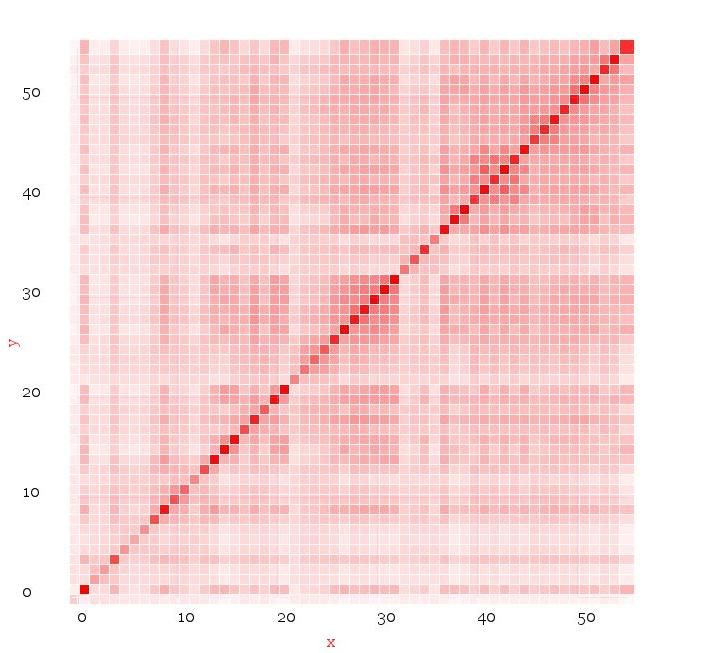
\includegraphics[width=120mm]{ReportMedia/CovariancePre.jpg}\\
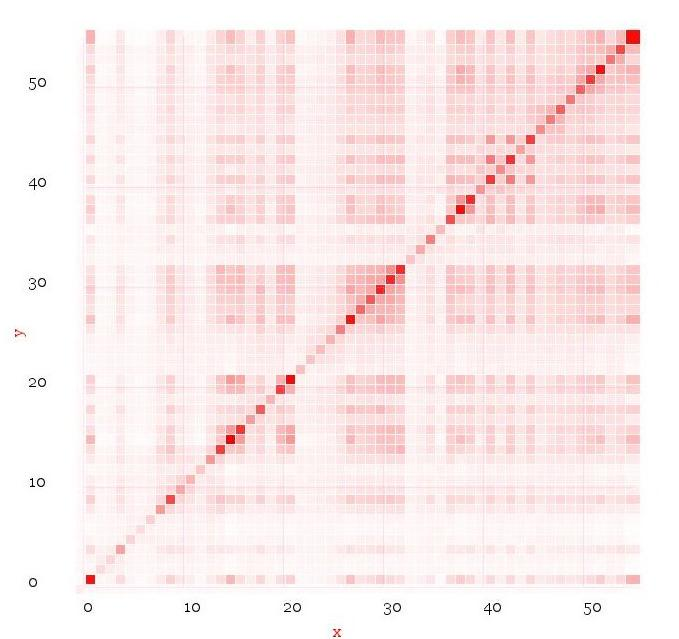
\includegraphics[width=120mm]{ReportMedia/CovariancePost.jpg}

\subsection{Answer distribution}
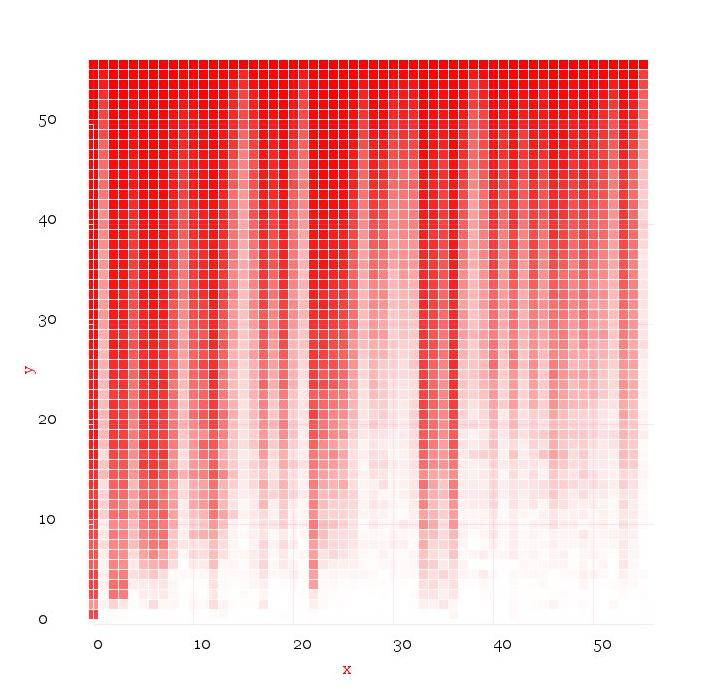
\includegraphics[width=120mm]{ReportMedia/AnswerDistribution.jpg}

\newpage
\section{Tests for Univariate Normality}
\subsection{Evidence}
\subsubsection{Jarque-Bera test}
\subsubsection{Normal probability plot}
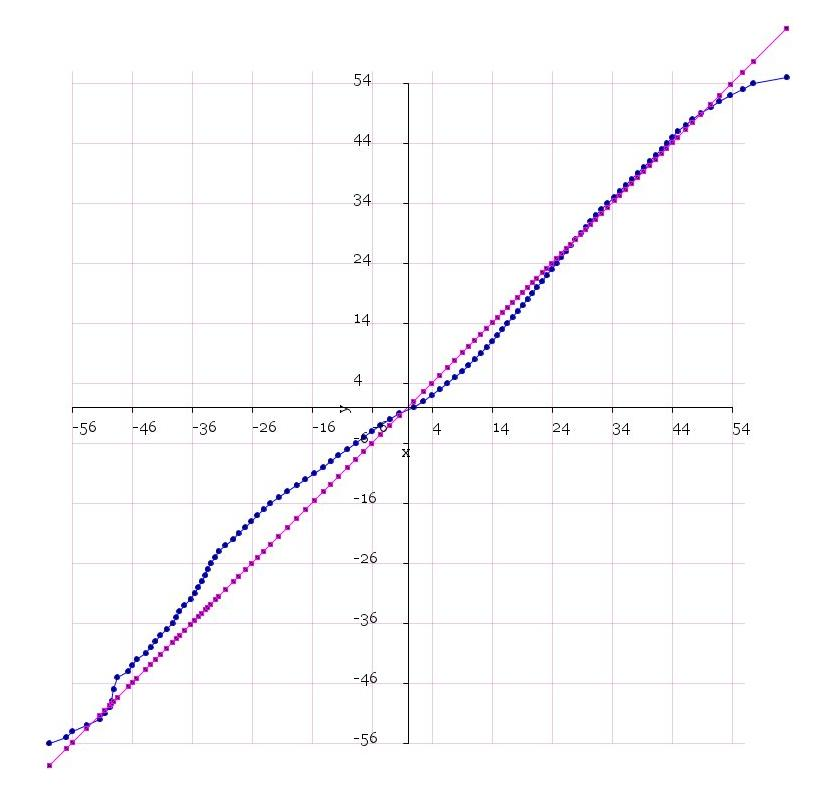
\includegraphics[width=120mm]{ReportMedia/NormalProbabilityPlotImprovement.jpg}
\subsection{Summary}
\newpage
\section{Tests for variable independence}
\subsection{Chi-square test}
\textbf{Null hypothesis: Area and Improvement are NOT related.} \\
 For \textbf{area vs. improvement}\\
 Chi-Square statistic = 56499.4692602837\\
 X2 = 9652.9739\\
 Degrees of freedom = 9426\\
 \textbf{Null hypothesis rejected}\\c
\\
\textbf{Null hypothesis: Area and Pre-Score are NOT related.}\\
 For \textbf{area vs. pre-score}\\
 Chi-Square statistic = 58665.7089390644\\
 X2 = 8062.2959\\
 Degrees of freedom = 7855\\
 \textbf{Null hypothesis rejected}\\
\\
\textbf{Null hypothesis: Area and Post-Score are NOT related.}\\
 For \textbf{area vs. post-score}\\
 Chi-Square statistic = 38567.0016158761\\
 X2 = 8062.2959\\
 Degrees of freedom = 7855\\
 \textbf{Null hypothesis rejected}\\
\\
\textbf{Null hypothesis: Language and Post-Score are NOT related.}\\
 For \textbf{language vs. post-score}\\
 Chi-Square statistic = 280.234448946825\\
 X2 = 96.2166\\
 Degrees of freedom = 75\\
 \textbf{Null hypothesis rejected}\\
\\
\textbf{Null hypothesis: Language and Improvement are NOT related.}\\
 For \textbf{language vs. improvement}\\
 Chi-Square statistic = 232.464548410971\\
 X2 = 113.1452\\
 Degrees of freedom = 90\\
 \textbf{Null hypothesis rejected}\\
\\
\textbf{Null hypothesis: Language and Pre-Score are NOT related.}\\
 For \textbf{language vs. pre-score}\\
 Chi-Square statistic = 277.85501653079\\
 X2 = 96.2166\\
 Degrees of freedom = 75\\
 \textbf{Null hypothesis rejected}\\

\newpage
\section{Prediction}
\subsection{Decision Trees}
\subsection{Bayes classifier}
\subsection{Density estimators}
\subsubsection{Naive Bayes density}
\subsubsection{Kernel density estimation}
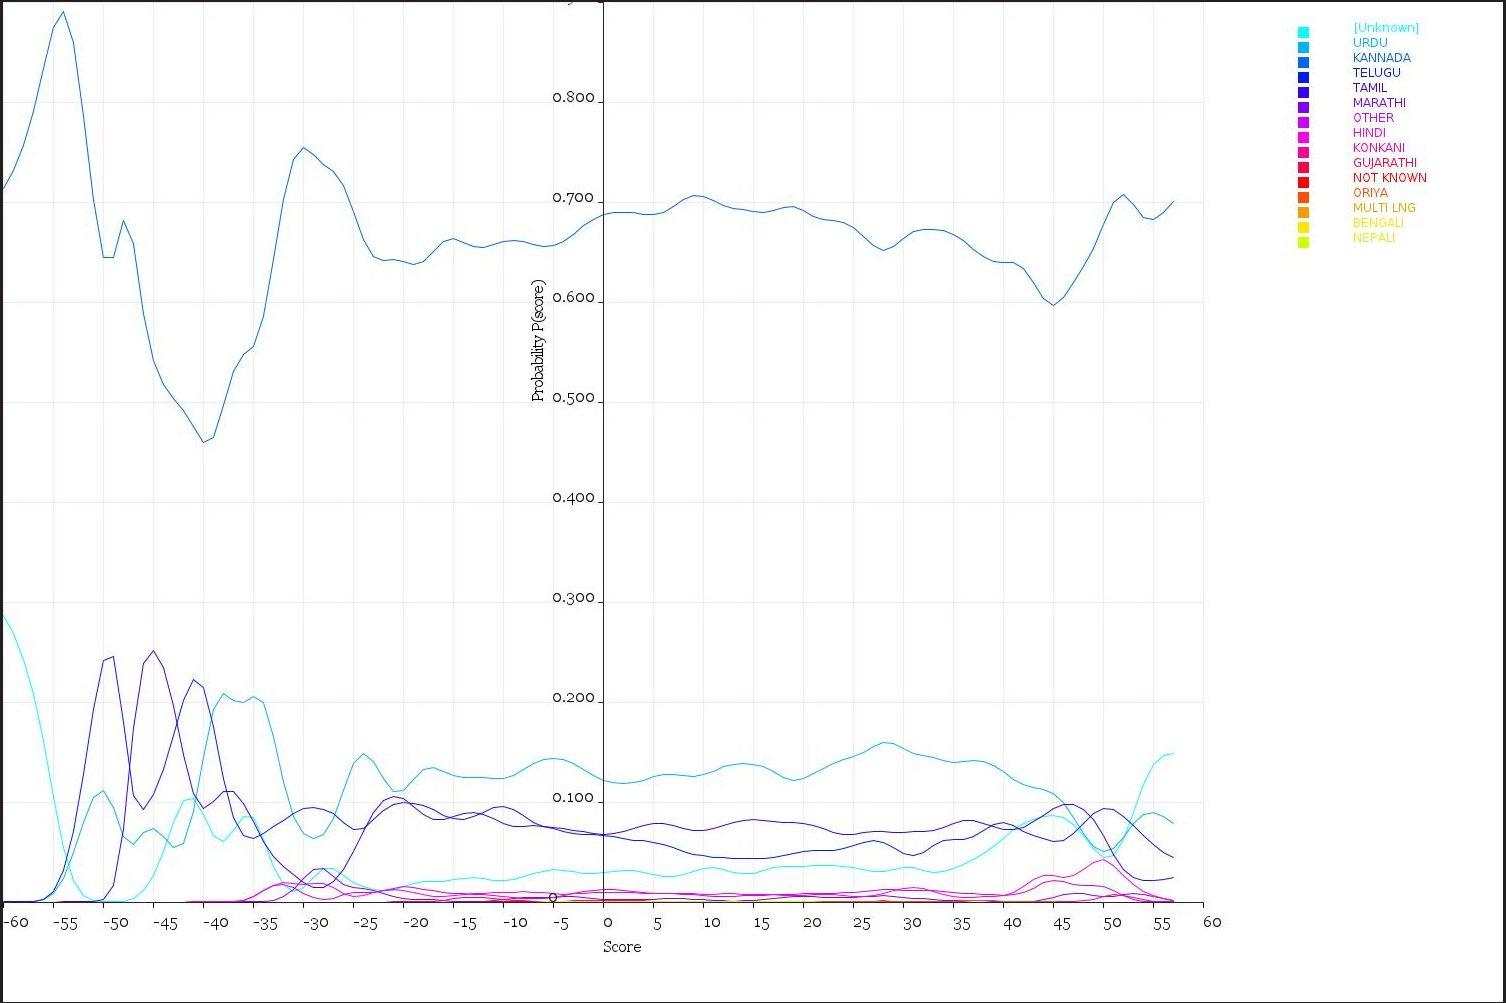
\includegraphics[width=160mm]{ReportMedia/BayesLanguageFromImprovement.jpg}
\newpage
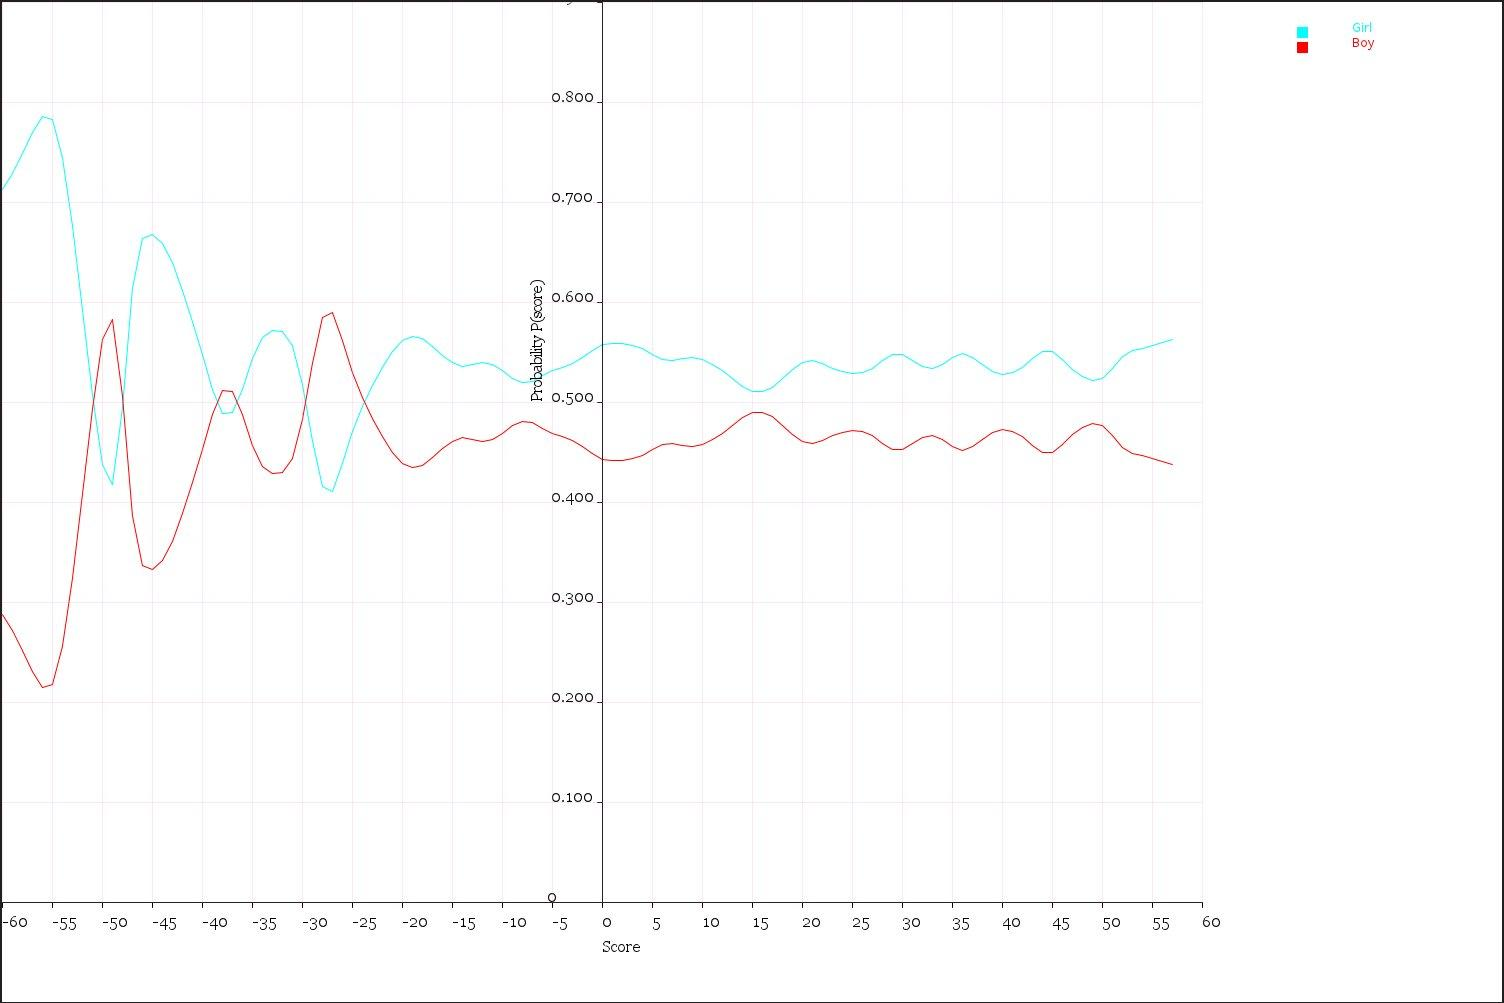
\includegraphics[width=160mm]{ReportMedia/BayesGenderFromImprovement.jpg}

\newpage
\section{Dimension reduction/Factor analysis}
\subsection{Principal Component Analysis}

\newpage
\section{Technical notes}

\end{document} 
